\documentclass[paper=a4,fontsize=12pt]{scrartcl}
\usepackage{geometry}
\usepackage{graphicx}
\geometry{verbose, a4paper, tmargin=25mm, bmargin=25mm, lmargin=25mm, rmargin=25mm}

\usepackage[utf8]{inputenc}
\usepackage[ngerman]{babel}
\usepackage{fancyhdr} %Paket laden
\pagestyle{fancy} %eigener Seitenstil
\fancyhf{} %alle Kopf- und Fu�zeilenfelder bereinigen
\fancyhead[L]{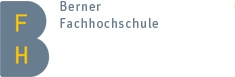
\includegraphics[width=3cm]{img/logo_bfh_de.jpg}} %Kopfzeile links
\fancyhead[C]{} %zentrierte Kopfzeile
\fancyhead[R]{Marco Berger, Andy Pollari} %Kopfzeile rechts
\renewcommand{\headrulewidth}{0.4pt} %obere Trennlinie
\fancyfoot[C]{\thepage} %Seitennummer
\renewcommand{\footrulewidth}{0.4pt} %untere Trennlinie

\makeatletter
\let\ps@plain\ps@fancy 
\makeatother

\begin{document}
\title{Abstract - Bildverschlüsselung mit Matlab}
\author{Marco Berger, Andy Pollari}
\date{14.01.2015}
\maketitle
% nur 10-12 Zeilen text, für einen Manager verständlich
Kryptographische Verschlüsselungen werden in der heutigen Zeit immer wichtiger.
Diese Arbeit hat sich das Ziel gesetzt, zu untersuchen, ob sich Matlab für gängige Verschlüsselungsverfahren 
angewandt auf JPG Bilder eignet.
Erst haben wir eine symetrische Verschlüsselung implementiert und untersucht. 
Danach haben wir die selben Untersuchungen auf eine asymetrische Verschlüsselung gemacht.
% Dabei wird einerseits eine symetrische und andererseits eine asymetrische Verschlüsselung angewandt.
Untere Untersuchen beziehen sich auf die Performance der Verschlüsselugen, Wiedererkennbarkeit der verschlüsselten Bilder
und ob die verschlüsselten Bilder gespeichert und von einem gewöhnlichen Bildbetrachter angesehen werden können.
Dabei stiessen wir auf grosse Unterschiede bei der gewählten symetrischen und der gewählten asymetrischen Verschlüsselung.
% Interessant dabei sind Fragen zur Performance der Verschlüsselungen, Wiedererkennbarkeit der verschlüsselten Bilder
% oder ob die verschlüsselte Bild gespeichert und von einem gewöhnlichen Bildbetrachter angesehen werden kann.
\newpage
\end{document}